\documentclass{book}

\usepackage[utf8]{inputenc}
\usepackage[T1]{fontenc}
\usepackage[francais]{babel}
\usepackage{graphicx} 
\usepackage{fancyref}
\usepackage{hyperref}
\usepackage{url}


\title{%
  Projet de Sciences des Données \\
  \large Explotation d'images satellites haute-résolution \\pour la prevision d'indicateurs socio-économiques \\
    }

\author{\textsc{Youcef} - \textsc{Kacer}}
\date{25 Aout 2016}

\begin{document}
 
\maketitle

\tableofcontents

\frontmatter
\chapter{Introduction}
Ce document présente le projet de sciences des données que je compte développer, dans le cadre de la validation du CES Data Scientist à Telecom-Paristech \cite{cesds}.\\
Ce projet consiste à exploiter des images satellitaires haute-résolution afin d'en extraire des indicateurs socio-économiques.\\
En effet, évaluer la densité démographique d'un pays, par exemple, peut représenter un co\^{u}t non négligeable en terme de 
recensement. Or utiliser des images aériennes et leurs caractéristiques permettrait de prédire la population présente à moindre co\^{u}t.
En effet, les \og edges \fg{} des routes et des batiments caractérisent les zones urbaines et donc les zones à forte population, alors que
les champs et les for\^{e}ts caractérisent des zones faiblement peuplées.\\

\mainmatter
\chapter{Images exploitées}

Les images à exploiter proviennent du satellite Landsat 8 de la NASA et sont libres d'accès \cite{landsat8}. Ce satellite scanne tout le globe terrestre 
tous les 16 jours, ce depuis 2013. Ces images permettent donc non seulement d'étudier une zone à un moment donnée mais aussi d'étudier son évolution sur
une période donnée (entre 2013 et 2016, on aurait donc 91 couvertures d'une même zone).\\
Ces images sont très riches dans la mesure où elles présentent en tout 11 canaux, 9 dans le visible et 2 dans l'infra-rouge. Donc en plus des caractéristiques de formes, le niveau des images doit pouvoir nous renseigner sur 
la nature des materiaux et des objets présents au sein d'une zone (métal ou végétation par exemple), les canaux infra-rouges pourront très certainement
quantifier la présence humaine.\\
Certaines combinaisons bien spécifiques de bandes peuvent apporter de l'information, comme le montre le tableau \ref{combinaison}
tiré de \cite{esri}:
\begin{table}
\begin{center}
\begin{tabular}{|c|c|c|c|}
\hline
Natural Color & 4 , 3 , 2\\
\hline
False Color (urban) & 7 , 6 , 4\\
\hline
Color Infrared (vegetation) & 5 , 4 , 3\\
\hline
Agriculture & 6 , 5 , 2\\
\hline
Atmospheric Peration & 7 , 6 , 5\\
\hline
Healthy Vegetation & 5 , 6 , 2\\
\hline
Land/Water & 5 , 6 , 4\\
\hline
Natural With Atmospheric Removal & 7 , 5 , 3\\
\hline
Shortwave Infrared & 7 , 5 , 4\\
\hline
Vegetation Analysis & 6 , 5 , 4\\
\hline
\end{tabular}
\end{center}
\caption{Combinaisons possibles à 3 canaux}
\label{combinaison}
\end{table}
\clearpage
Ces bandes couvrent approximativement un périmètre de 185km dans la direction Nord-Sud et 185km
dans la direction Est-Ouest, pour une résolution de 30 mètres (soit des images de ~8000x8000 pixels). Cette
résolution équivaut à la demi-longueur d'un terrain de football, ce qui ne sera pas
suffisant pour récupérer les edges des batiments et autres structures, c'est pour cela qu'on envisagera de coupler nos images
satellitaires à l'exploitation des images couleur de Google Earth.\\
Les figures \ref{band2},\ref{band3},\ref{band4} présentent respectivement les bandes 2,3 et 4 d'un dataset que nous
avons pu télécharger depuis \cite{landsat8}, et pris autour de la ville
de \begin{itshape}Grenada (Espagne)\end{itshape}

\begin{figure}[H]
\begin{center}
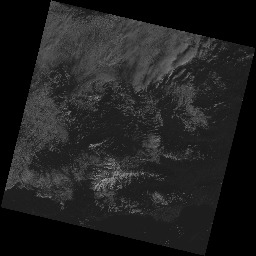
\includegraphics[scale=0.8]{LC82000342015021LGN00_B2r.jpg}
\end{center}
\caption{image Lansat-8 (bande 2), région autour de $Grenada$ $(Espagne)$}
\label{band2}
\end{figure}

\begin{figure}[H]
\begin{center}
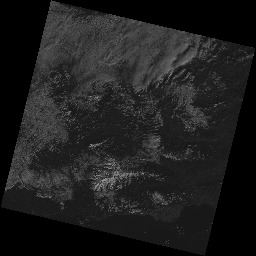
\includegraphics[scale=0.8]{LC82000342015021LGN00_B3r.jpg}
\end{center}
\caption{image Lansat-8 (bande 3), région autour de $Grenada$ $(Espagne)$}
\label{band3}
\end{figure}

\begin{figure}[H]
\begin{center}
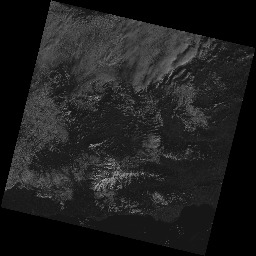
\includegraphics[scale=0.8]{LC82000342015021LGN00_B4r.jpg}
\end{center}
\caption{image Lansat-8 (bande 4), région autour de $Grenada$ $(Espagne)$}
\label{band4}
\end{figure}

\clearpage

\chapter{Méthode d'apprentissage}

L'idée serait de s'intéresser à une certaine zone (un pays par exemple), dont on aurait l'indicateur de densité de population (valeur 
à prédire) pour un grand ensemble de communes du pays.\\
On pourra alors récupérer plusieurs images satellitaires quadrillant ce pays, et attribuer à chacune d'elles
sa valeur de densité de population (on doit pouvoir utiliser la latitude et la longitude d'une image pour retrouver la commune concernée).\\
Ainsi, on récupère un ensemble classique d'images labelisées par sa densité de population.\\
Ensuite, on pourra extraire des descripteurs de ces images (histogramme orienté du gradient \cite{Dalal05histogramsof}, entre autre)
auquels on appliquera un algorithme de regression supervisé (la valeur à prédire, la densité de
population, est plut\^{o}t continue que discrète).\\
On aurait donc un modèle de classification capable de prédire la densité de population d'une zone en fonction d'images satellites.\\
On pourra alors tester la généralisation du classifieur, en s'intéressant à d'autres pays.\\

\chapter{Outils pour le stockage, le calcul et la visualisation}

Si l'on s'intéresse à un territoire grand comme la France, on doit s'attendre à récupérer un total de 49 datasets 
pour quadriller cette zone \ref{quadrillage}\\
\begin{figure}[H]
\begin{center}
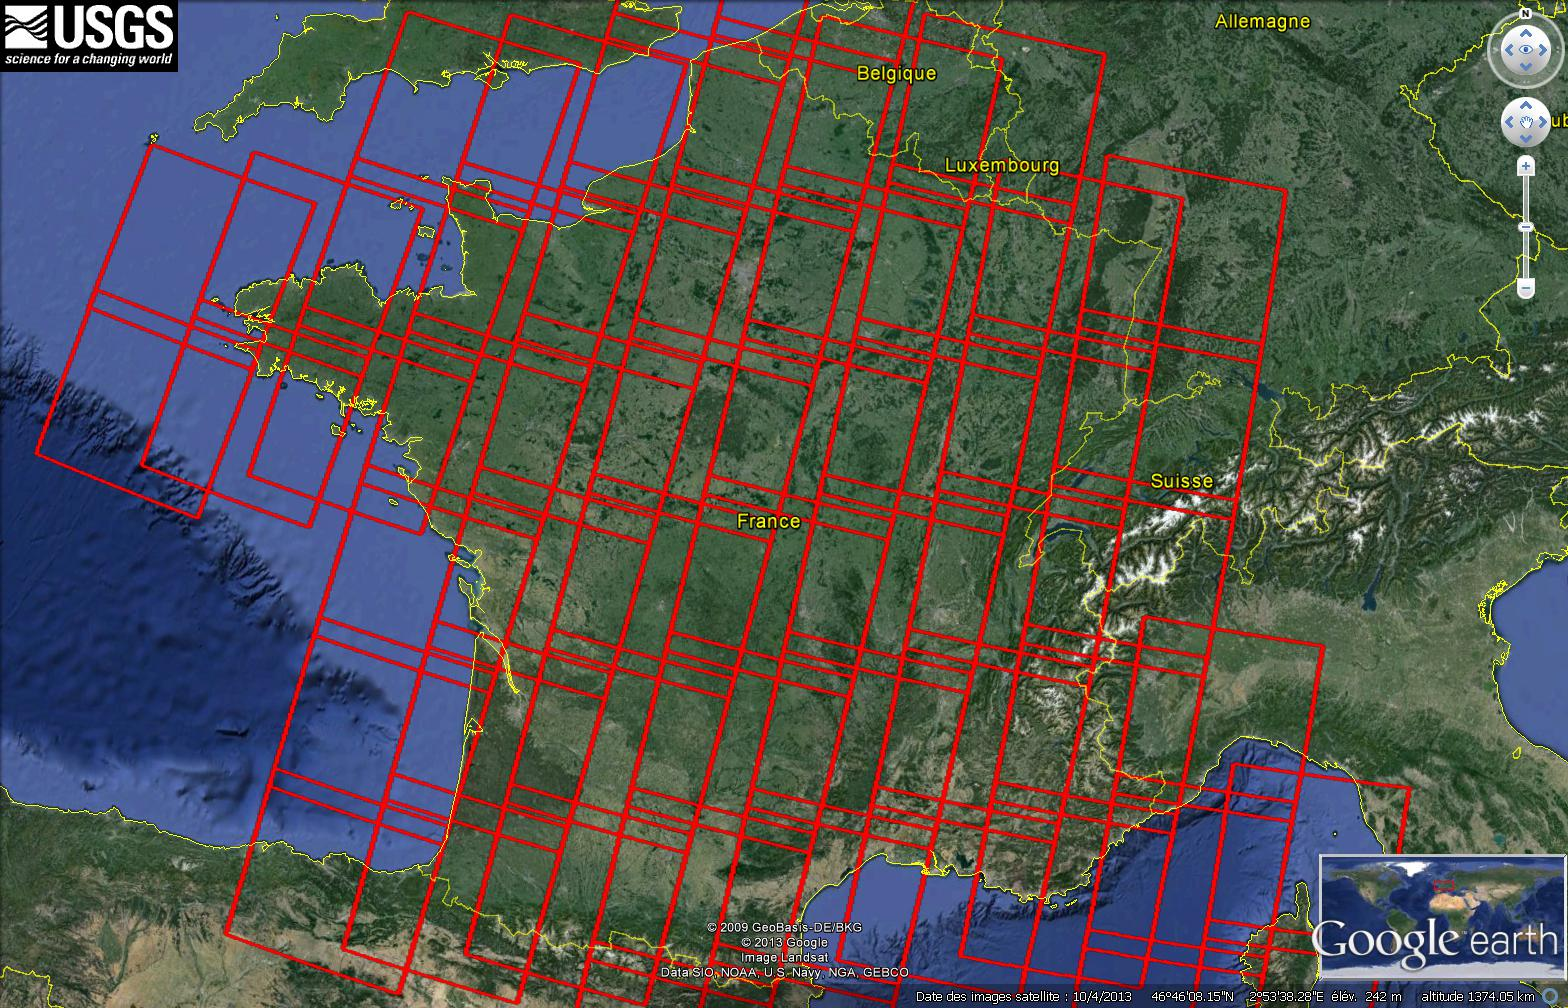
\includegraphics[scale=0.25]{emrpise_france_landsat8.jpg}
\end{center}
\caption{Quadrillage de la France par Landsat-8 \cite{geosud}}
\label{quadrillage}
\end{figure}
\clearpage

Chaque dataset compte les 11 bandes évoquées plus haut, mais aussi une image d'information de 
qualité renseignant pour chacun des pixels, la présence ou non de nuage, la présence ou non de mers ainsi que la 
présence ou non de neige.\\
Ainsi, chaque dataset mesure approximativement 1Go, on donc aurait une quantité totale de \begin{bf}49Go\end{bf} . 
Des descripteurs comme les 
hitogrammes orientés du gradient (pour une taille de block 16 pixels , une taille de cellule de 4, un recouvrement de 4)
pourraient multiplier cette quantité par un facteur 8, soit \begin{bf}392Go\end{bf}, ce qui ne tiendrait pas 
en mémoire vive.
Les images seront donc stockées sur HDFS \cite{White:2009:HDG:1717298} (soit en mode \og single-node cluster \fg, 
soit en mode \og multi-node cluster \fg via le cluster de Telecom ParisTech), cela permettra
d'extraire les descripteurs par Map/Reduce. Les descripteurs seront aussi stockés de manière distribuée, via une table HBASE afin de 
pouvoir effectuer des requ\^{e}tes et vérifier les valeurs calculées.\\
Une fois les descripteurs calculés, on utilisera la librairie de Machine Learning MLlib de Spark \cite{Meng:2016:MML:2946645.2946679}, 
dédiée à l'apprentissage sur données distribuées dans HDFS.
Pour la regression, cette librairie ne permet cependant que les regressions linéaires 
(soit par moindres carrés, par Ridge ou par Lasso) et les regressions logistiques (pas de SVM regressif).\\
On testera toutes ces méthodes pour en analyser les erreurs en cross-validation.\\
Enfin, pour la visualisation des resultats, on proposera une page html utilisant la librairie javascript 
D3 \cite{Jain:2014:DVD:2667432.2667451} pour l'affichage de la carte de densité de population. Cette interface web sera aussi
intéractive que possible afin de permettre des zooms mais aussi l'observation de la densité de population sur une année antérieure.

\clearpage

\backmatter

\listoftables

\listoffigures

\bibliographystyle{alpha}
\bibliography{biblio}

\end{document}